\documentclass{beamer}
\usepackage[italian]{babel}
\usepackage[utf8]{inputenc}
\usepackage[T1]{fontenc}
\usepackage{graphicx}
\usepackage{tikz}
\usepackage{booktabs}
\usepackage{hyperref}
\usepackage{eurosym}

\usetheme{AnnArbor}
%\useoutertheme{miniframes}
\setbeamercovered{dynamic}


\institute[DICAM - UNITN]{\normalsize{Universit\`a degli Studi di Trento}\\\footnotesize{Dipartimento di ingegneria civile, ambientale e meccanica\\Laurea Magistrale in Ingegneria Civile\\ Anno Accademico 2018/2019}}
\logo{\includegraphics[width = 15mm]{images/logo}}

\title[Progetto di una fognatura pluviale]{Progetto di una fognatura pluviale a Pergine Valsugana}
\subtitle{Corso di Costruzioni Idrauliche}

\author[Franzoi - Rebellato]{%
  \texorpdfstring{%
    \begin{columns}
      \column{.3333\linewidth}
      \centering
      \textbf{Studenti}: \\  Matteo Franzoi \\ Andrea Rebellato
      \column{.3333\linewidth}
      \centering
      \textbf{Docente}: \\ Prof. Riccardo Rigon
       \column{.3333\linewidth}
      \centering
        \textbf{Esercitatori}: \\ Niccolò Tubini \\ Daniele Della Torre
    \end{columns}
}%
 {}%
}%
\date{giugno 2019}
%
%
%
\setbeamertemplate{background canvas}{%
\begin{tikzpicture}[remember picture,overlay]
\shade[top color=gray, bottom color=white]
  (current page.north west)
     rectangle
  (current page.south east);
\end{tikzpicture}%     
}
\setbeamertemplate{navigation symbols}{}

\newcommand{\nologo}{\setbeamertemplate{logo}{}}
%
%
%
\begin{document}
{%
\usebackgroundtemplate{%
 \tikz \node[opacity=.5] {\includegraphics[height=1\paperheight, width=\paperwidth]{images/pioggia}};
}
\begin{frame}
    \maketitle
\end{frame}
}

\begin{frame}
    \frametitle{Indice}
    \tableofcontents
\end{frame}



\section{Inquadramento}
\begin{frame}
 \frametitle{Scelta dell'area}
 \begin{columns}
 \begin{column}{.5\textwidth}
  \begin{figure}
   \centering
   \includegraphics[width=\linewidth]{images/area}
  \end{figure}
  \end{column}

 \begin{column}{.5\textwidth}
  \begin{itemize}[<+->]
   \item Pergine Valsugana, nei pressi di Ponte Regio
   \item a lato del torrente Fersina
   \item superficie di circa $57\,ha$
   \item comprende in parte la zona residenziale e in parte la zona industriale
  \end{itemize}
 \end{column}
 \end{columns}
 
\end{frame}

\begin{frame}
 \frametitle{Analisi dell'area}
 
 \begin{columns}
  \begin{column}{.5\textwidth}
   \begin{figure}
    \centering
    \includegraphics[width=\linewidth]{images/analisi_area}
   \end{figure}
  \end{column}
  
  \begin{column}{.5\textwidth}
   \begin{itemize}[<+->]
    \item pendenza non trascurabile in direzione EST-OVEST
    \item altitudine massima di $484\,m$
    \item altitudine minima di $461\,m$
    \item pendenza del piano stradale a favore del torrente Fersina
    \item larghezza delle strade sufficiente per l'affiancamento planimetrico delle reti
   \end{itemize}
  \end{column}
 \end{columns} 
\end{frame}

\section{Progetto della fognatura pluviale}
\begin{frame}
 \frametitle{Ipotesi progettuali}
 \begin{itemize}[<+->]
  \item rete a maglia aperta
  \item collettore di scarico nel torrente Fersina
  \item acquedotto posto a $1.20\,m$ sotto il piano stradale
  \item generatrice superiore della fognatura posta a $30\,cm$ al di sotto dell'acquedotto
  \item pendenza iniziale pari alla pendenza del piano campagna
 \end{itemize}
\end{frame}

\begin{frame}
 \frametitle{Creazione della rete su QGIS}
 
 \begin{columns}
  \begin{column}{.5\textwidth}
   \begin{figure}
    \centering  
    \begin{overprint}
     \onslide<1>\includegraphics[width=\linewidth]{images/junctions}
     \onslide<2>\includegraphics[width=\linewidth]{images/outfall}
     \onslide<3>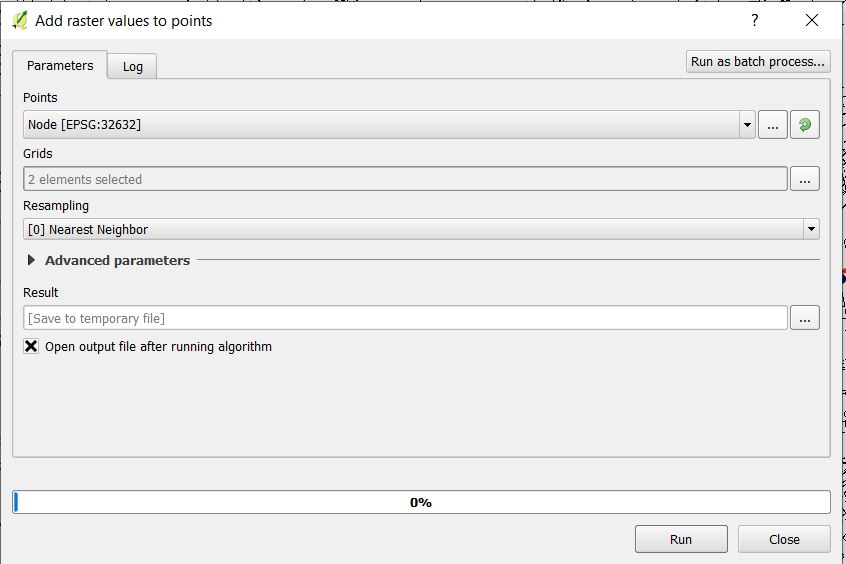
\includegraphics[width=\linewidth]{images/calcolo_quote_nodi}
     \onslide<4>\includegraphics[width=\linewidth]{images/conduits}
    \end{overprint}
   \end{figure}
  \end{column}
  
  \begin{column}{.5\textwidth}
   \begin{itemize}[<+->]
    \onslide<1>\item posizionamento delle $30$ \emph{junctions}, principalmente sulle intersezioni stradali
    \onslide<2>\item posizionamento dell'\emph{outfall} in corrispondenza del torrente Fersina
    \onslide<3> \item calcolo delle quote relative ai nodi
    \onslide<4> \item creazione dei 30 tubi
   \end{itemize}
  \end{column}
 \end{columns}
\end{frame}

\begin{frame}
 \frametitle{Creazione della rete su QGIS}
 
 \begin{columns}
  \begin{column}{.5\textwidth}
   \begin{figure}
    \centering  
    \begin{overprint}
     \onslide<1>\includegraphics[width=\linewidth]{images/subcatchments}
     \onslide<2> 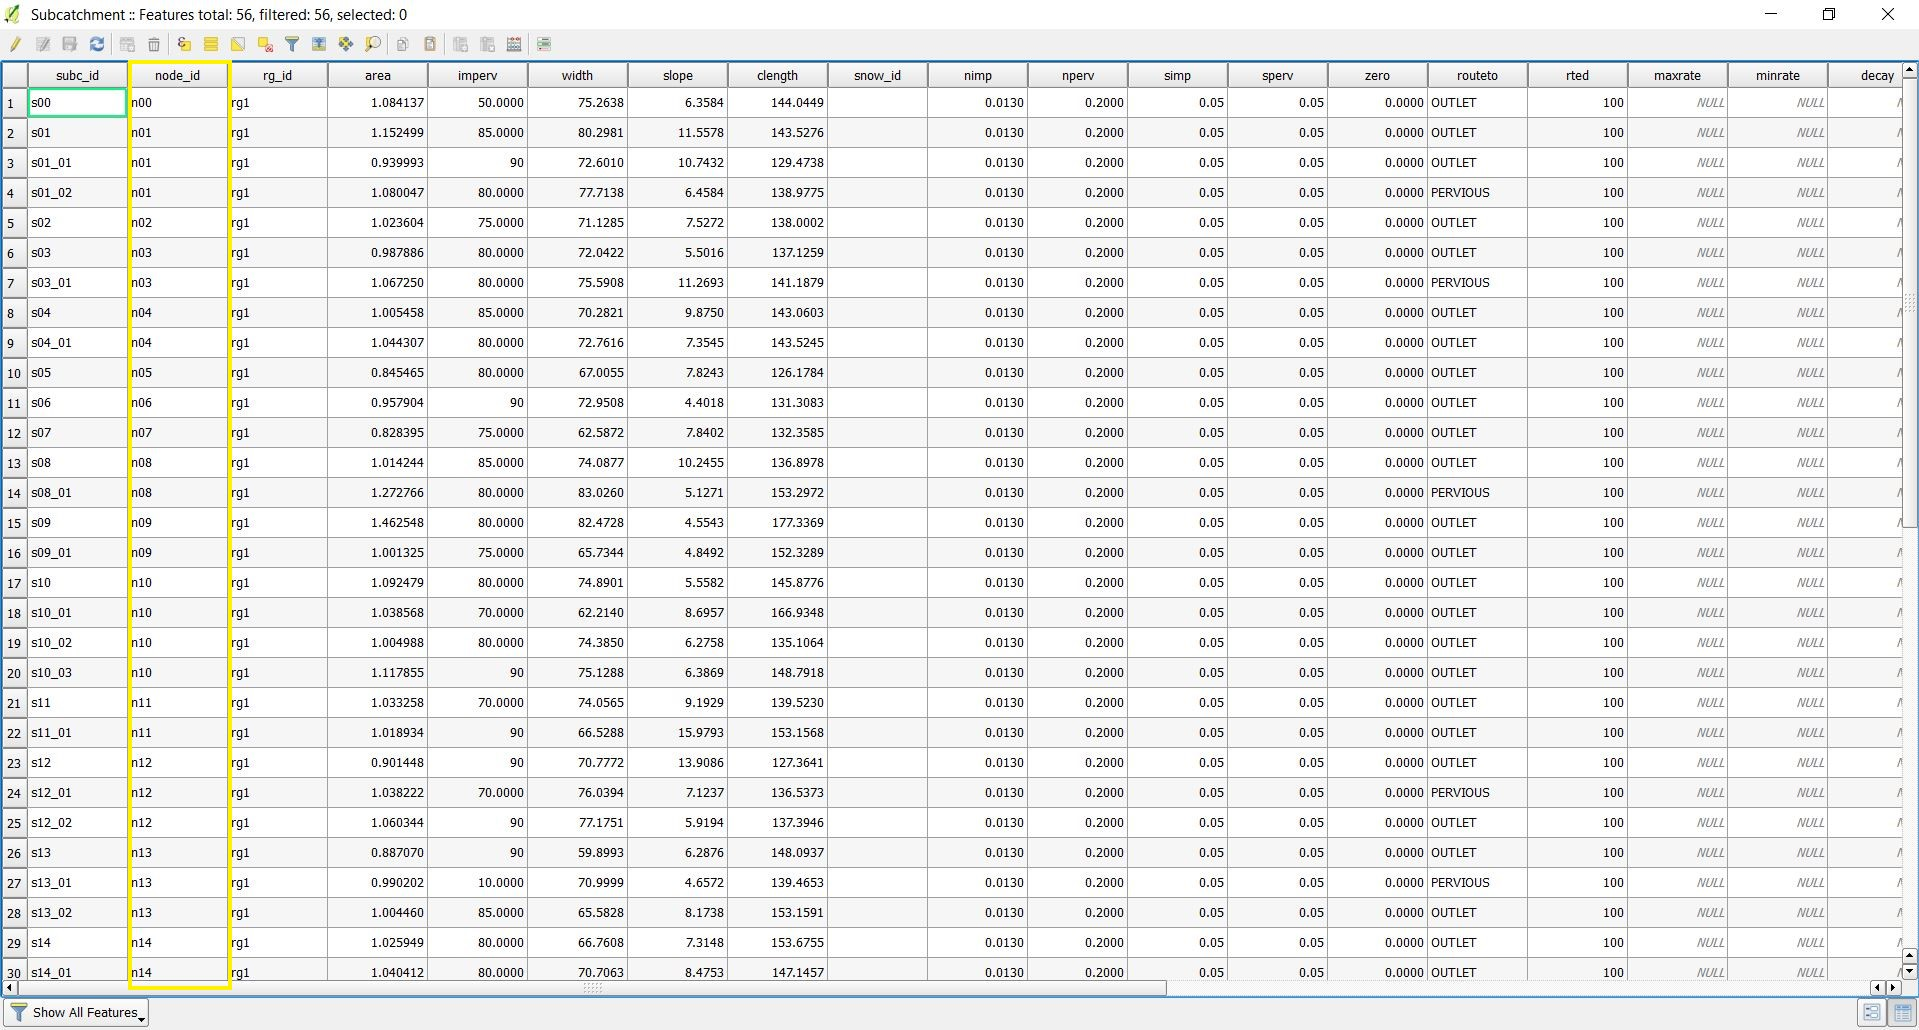
\includegraphics[width=\linewidth]{images/subcatchments_properties}
     \onslide<3> 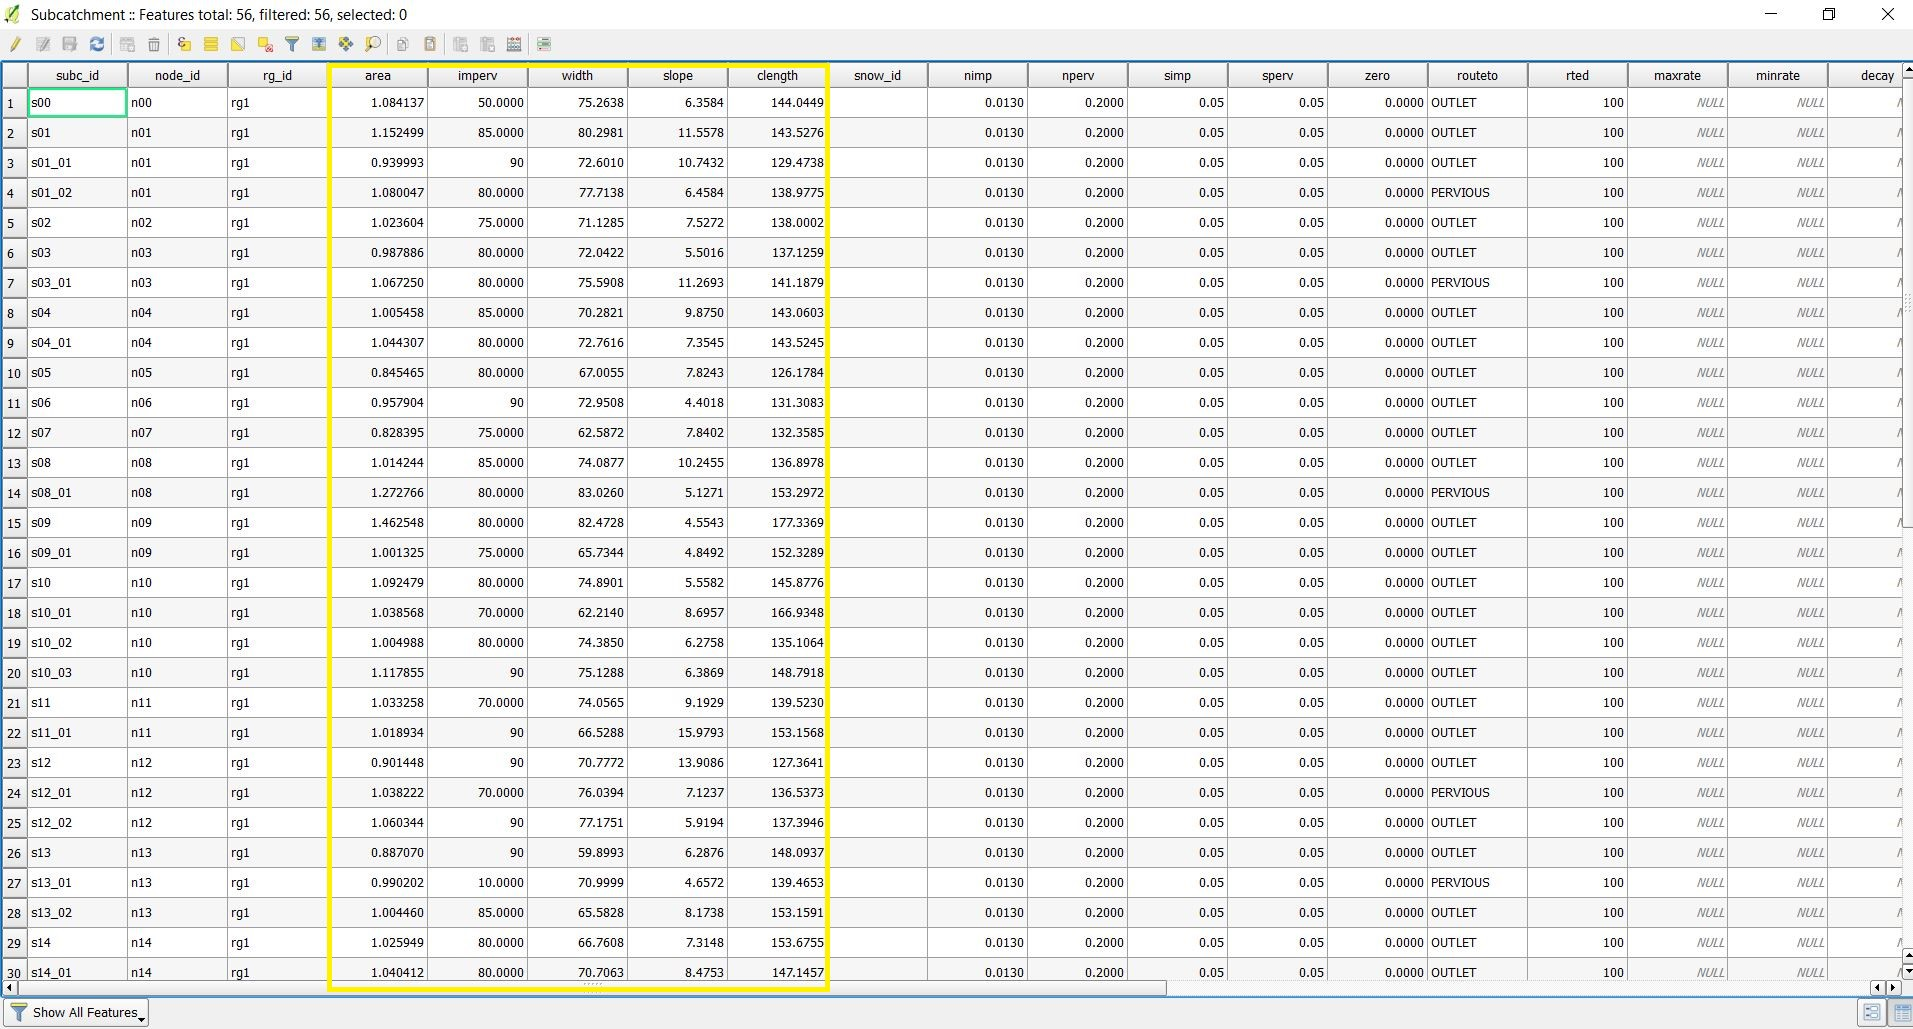
\includegraphics[width=\linewidth]{images/subcatchments_geometry}
    \end{overprint}
   \end{figure}
  \end{column}
  
  \begin{column}{.5\textwidth}
   \begin{itemize}[<+->]
    \onslide<1>\item creazione dei sottobacini il più possibile omogenei di area $1\,ha$ circa
    \onslide<2> \item assegnazione del nodo di scarico di ogni sottobacino
    \onslide<3> \item definizione delle caratteristiche geometriche di ogni sottobacino
   \end{itemize}
  \end{column}
 \end{columns}
\end{frame}

\begin{frame}
 \frametitle{Esportazione della rete con Giswater}
 Tramite il software \emph{Giswater} si esporta quanto fatto su QGIS in un file con estensione \emph{inp}, il quale verrà importato su \emph{SWMM}.
\end{frame}


%-------------------------------------------------------


\section{Analisi pluviometrica}
\begin{frame}
    \frametitle{Intensità di precipitazione}
    
    \begin{block}{Intensità di precipitazione}
     Si definisce \emph{intensità di precipitazione} la grandezza
     \begin{equation}
     \label{eq:intensita_precipitazione}
      J(t_p, T_r) = \dfrac{h(t_p, T_r)}{t_p} = a(T_r)\,t_p^{n-1}
     \end{equation}
    \end{block}
\end{frame}

\begin{frame}
 \frametitle{Stima dei parametri $a$ e $n$}
 
 Dall'analisi pluviometrica, in particolare dal tracciamento delle \emph{linee segnalatrici di possibilità pluviometrica}, si ricavano i valori dei parametri $a$ e $n$ relativi agli scrosci.
 \begin{table}
 \caption{Valori di $a$ e $n$ degli scrosci}
  \begin{tabular}{cccc}
  \toprule
  &         n &          a \\
  \midrule
  $T_r = 10\,y$  &  0.433588 &  33.437650 \\
  $T_r = 20\,y$  &  0.434880 &  37.914897 \\
  $T_r = 100\,y$&  0.436892 &  48.052780 \\
  \bottomrule
  \end{tabular}
 \end{table}

\end{frame}


\begin{frame}
 \frametitle{Calcolo delle intensità di precipitazione}
 Inserendo i valori di appena trovati all'interno della \eqref{eq:intensita_precipitazione} si ricavano le seguenti intensità:
  \small
    \begin{table}
    \caption{Intensità di precipitazione degli scrosci}
    \begin{tabular}{cccccc}
    \toprule
    &5 min &      10 min &      15 min &      20 min &      25 min \\ 
    \midrule
    $T_r = 10\,y$ &47.780861 &  29.880404 &  22.705529 &  18.686112 &  16.065279 \\
    $T_r = 20\,y$ &57.041849 &  35.478913 &  26.874315 &  22.067188 &  18.939039 \\
    $T_r = 100\,y$ &78.317726 &  48.303355 &  36.408581 &  29.791648 &  25.499248 \\
    \bottomrule
    \end{tabular}
    \end{table}
    che verranno utilizzate per la crezione della \emph{timeseries}.
\end{frame}

\section{Verifica della rete}
\begin{frame}
 \frametitle{Verifica della rete su SWMM}
 
 \begin{columns}
  \begin{column}{.5\textwidth}
  \begin{figure}
   \centering
   \begin{overprint}
    \onslide<1> 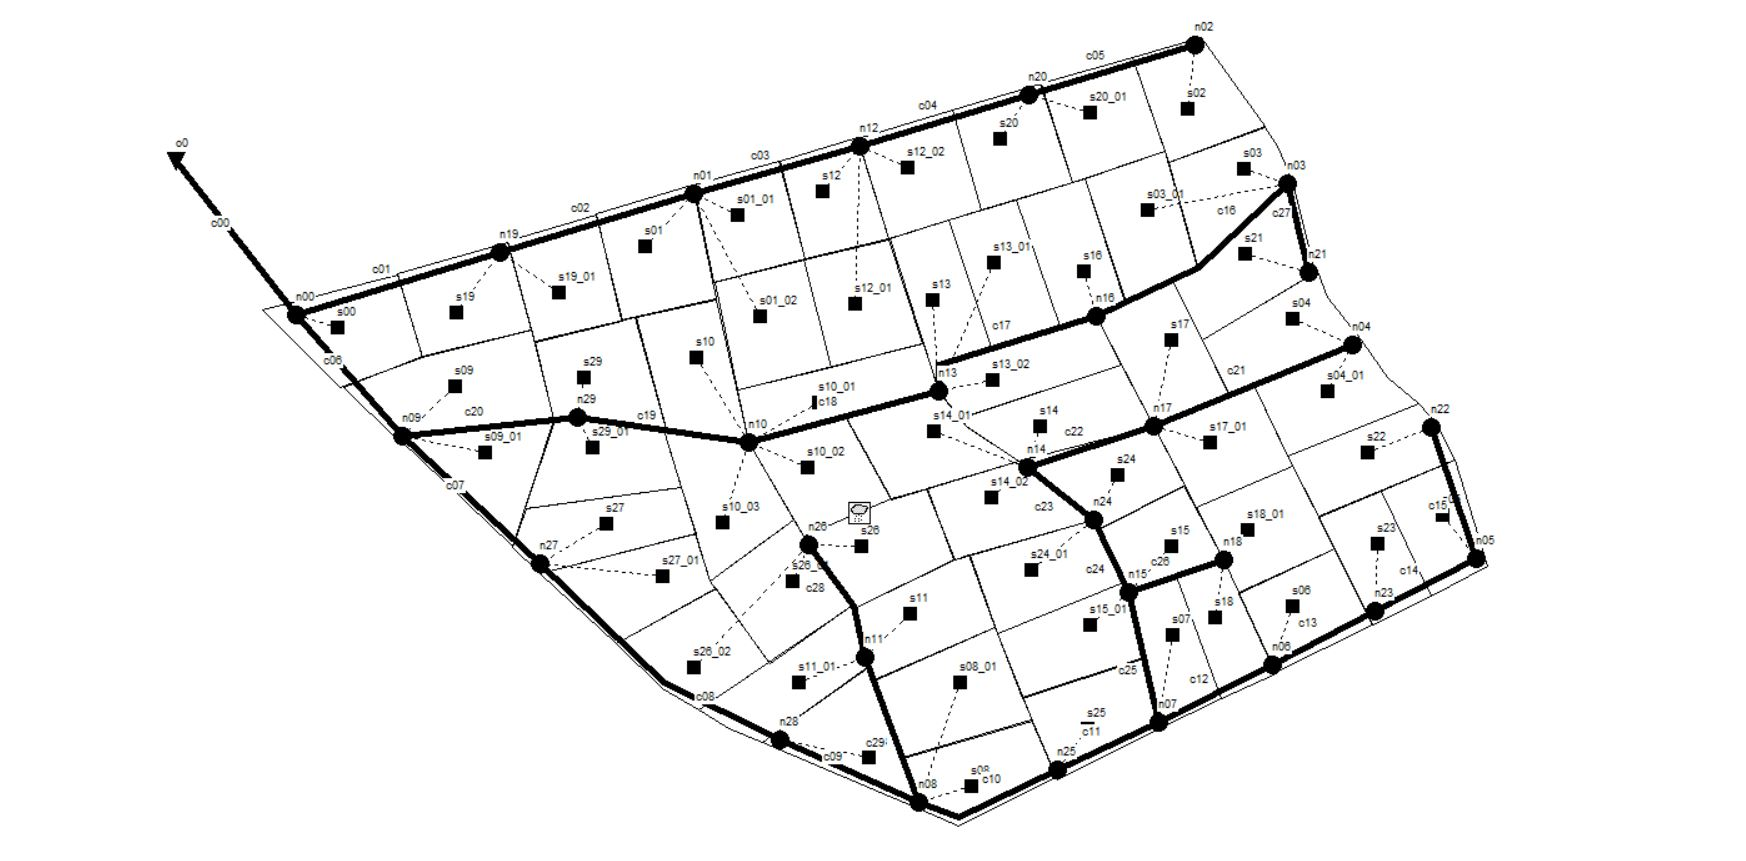
\includegraphics[width=\linewidth]{images/map}
    \onslide<2> \includegraphics[width=.98\linewidth]{images/timeseries}
    \onslide<3> 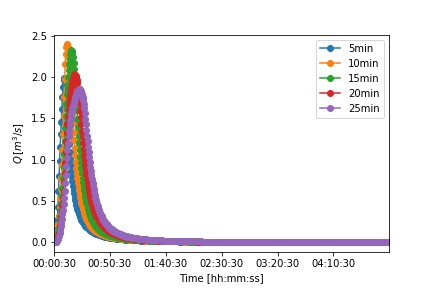
\includegraphics[width=\linewidth]{images/portata_massima}
   \end{overprint}
  \end{figure}   
  \end{column}
  
  \begin{column}{.5\textwidth}
   \begin{itemize}
   \onslide<1> \item importazione del progetto in \emph{SWMM}
   \onslide<2> \item creazione della \emph{timeseries}
   \onslide<3> \item calcolo della portata massima per ogni nodo attraverso i relativi notebook
  \end{itemize}
  \end{column}
 \end{columns}
\end{frame}

\begin{frame}
 \frametitle{Scelte progettuali}
 \begin{itemize}
  \item tubi e pezzi speciali in polietilene strutturato ECOPAL SN 8 (\url{https://www.oppo.it/materiali/tubi_raccordi/ecopal_tubi.html})
  \item coefficiente di Manning \[n = 0.011\]
  \item moto uniforme e stazionario definito dalla formula di Guckler - Strickler
  \[Q_{max} = k_s\,\Omega\,R_H^{2/3}\,i_f^{1/2}\]
  \item invertendo la formula per calcolare il diametro di prima approssimazione
  \[
   D = b\,\left[ \frac{2^{13/3}\,\frac{Q_{max}}{k_s\,i_f^{1/2}}}{(1-\frac{\sin \theta}{\theta})^{2/3}(\theta -\sin \theta)}\right]^{3/8}
  \]
  \[
   \theta = 2\, \cos^{-1} (1-G)
  \]
 \end{itemize}
\end{frame}

\begin{frame}
 \frametitle{Calcolo del diametro con jupyter}
    \begin{itemize}
     \item calcolo del diametro di prima approssimazione relativo alla condotta in studio attraverso i jupyter notebook
     \item arrotondamento del diametro trovato al diametro commerciale
    \end{itemize}
 
 \scriptsize
   \begin{table}
   \caption{DataFrame riassuntivo di ogni condotta}
    \begin{tabular}{lllllllll}
        \toprule
        Condotta & Portata [l/s] & Pendenza & Diametro &         G\\
        \midrule
        c00      &       2396.29 &    0.008 &    1.025 &  0.748977\\
        \bottomrule
         &   theta &        Rh &      tau & Criterio di autopulizia \\
         \midrule
          &  239.73 &  0.309144 &  24.2616 &                        Verificato! \\
        \bottomrule
    \end{tabular}    
   \end{table}
\end{frame}

\begin{frame}
 \frametitle{Verifica della rete su SWMM}
 
 \begin{columns}
  \begin{column}{.5\textwidth}
  \begin{figure}
   \centering
   \begin{overprint}
    \onslide<1> \includegraphics[width=\linewidth]{images/sostituzione_diametro}
    \onslide<2> 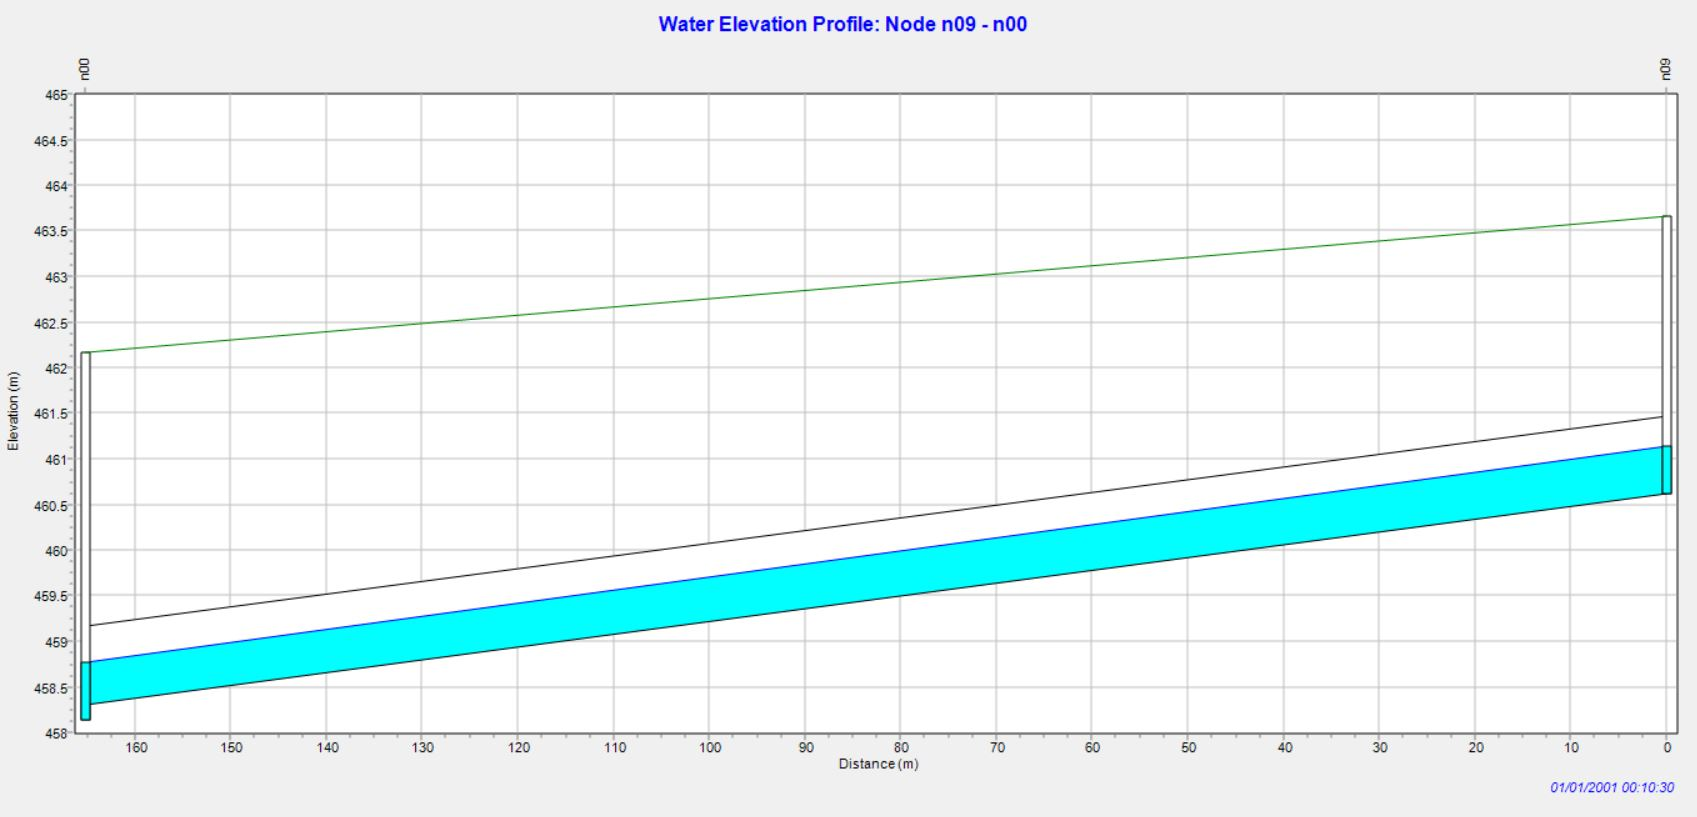
\includegraphics[width=.98\linewidth]{images/verifica_condotta}
   \end{overprint}
  \end{figure}   
  \end{column}
  
  \begin{column}{.5\textwidth}
   \begin{itemize}
   \onslide<1> \item sostituzione del diametro commerciale trovato all'interni di SWMM
   \item modifica della quota in funzione al diametro esterno della condotta
   \onslide<2> \item verifica della condotta su SWMM   
   \end{itemize}
  \end{column}
 \end{columns}
\end{frame}

\begin{frame}
 \frametitle{Verifica della rete su SWMM}
 
 \begin{columns}
  \begin{column}{.5\textwidth}
  \begin{figure}
   \centering
   \begin{overprint}
    \onslide<2> 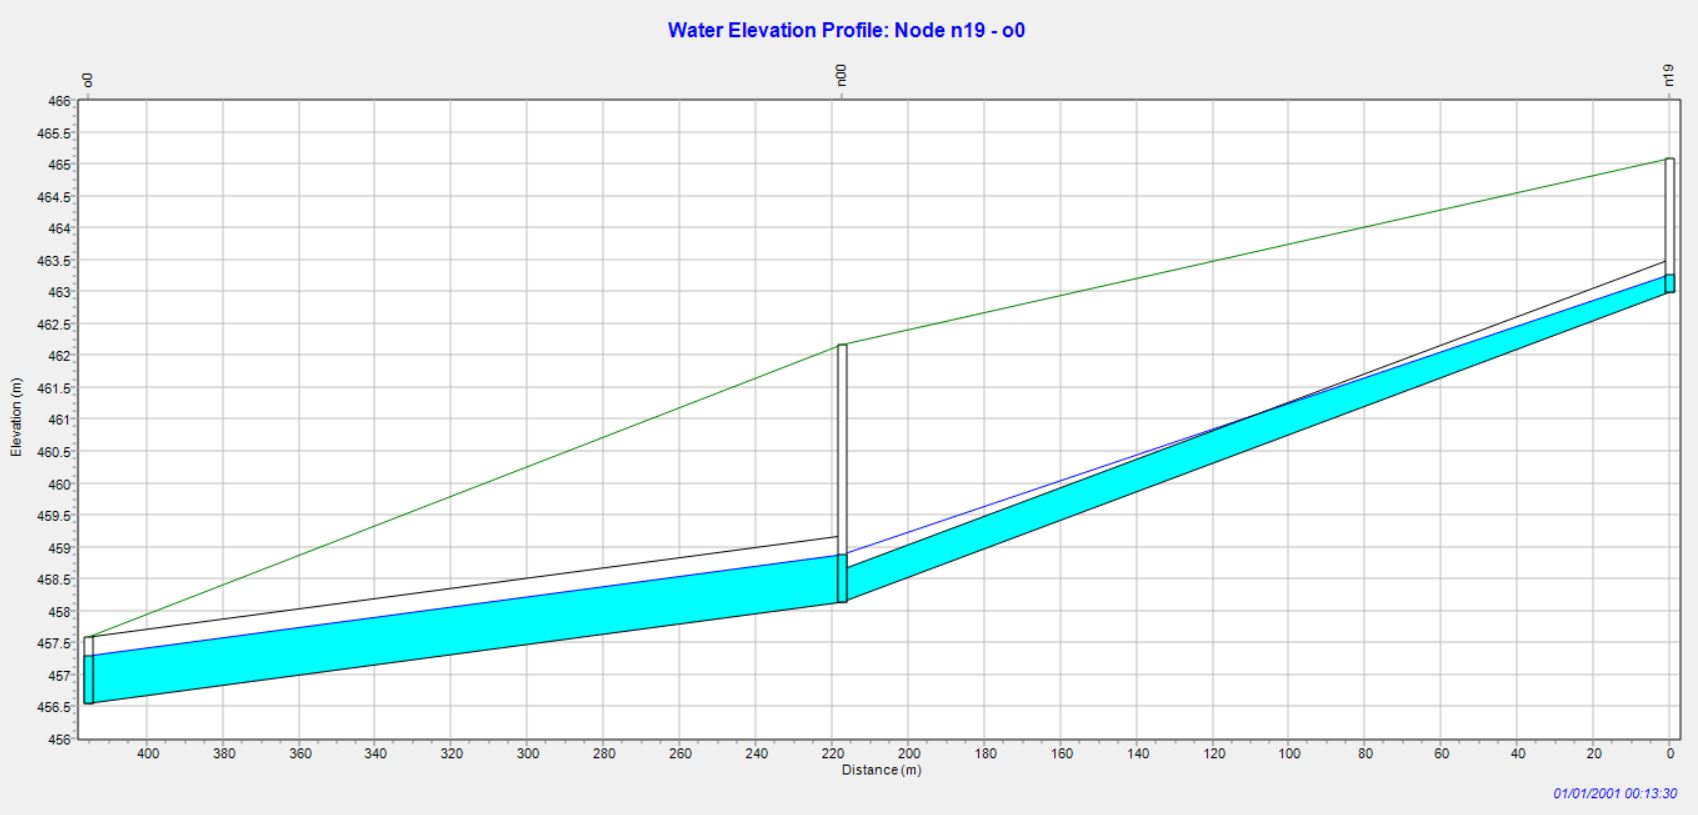
\includegraphics[width=\linewidth]{images/rigurgito}
    \onslide<3> 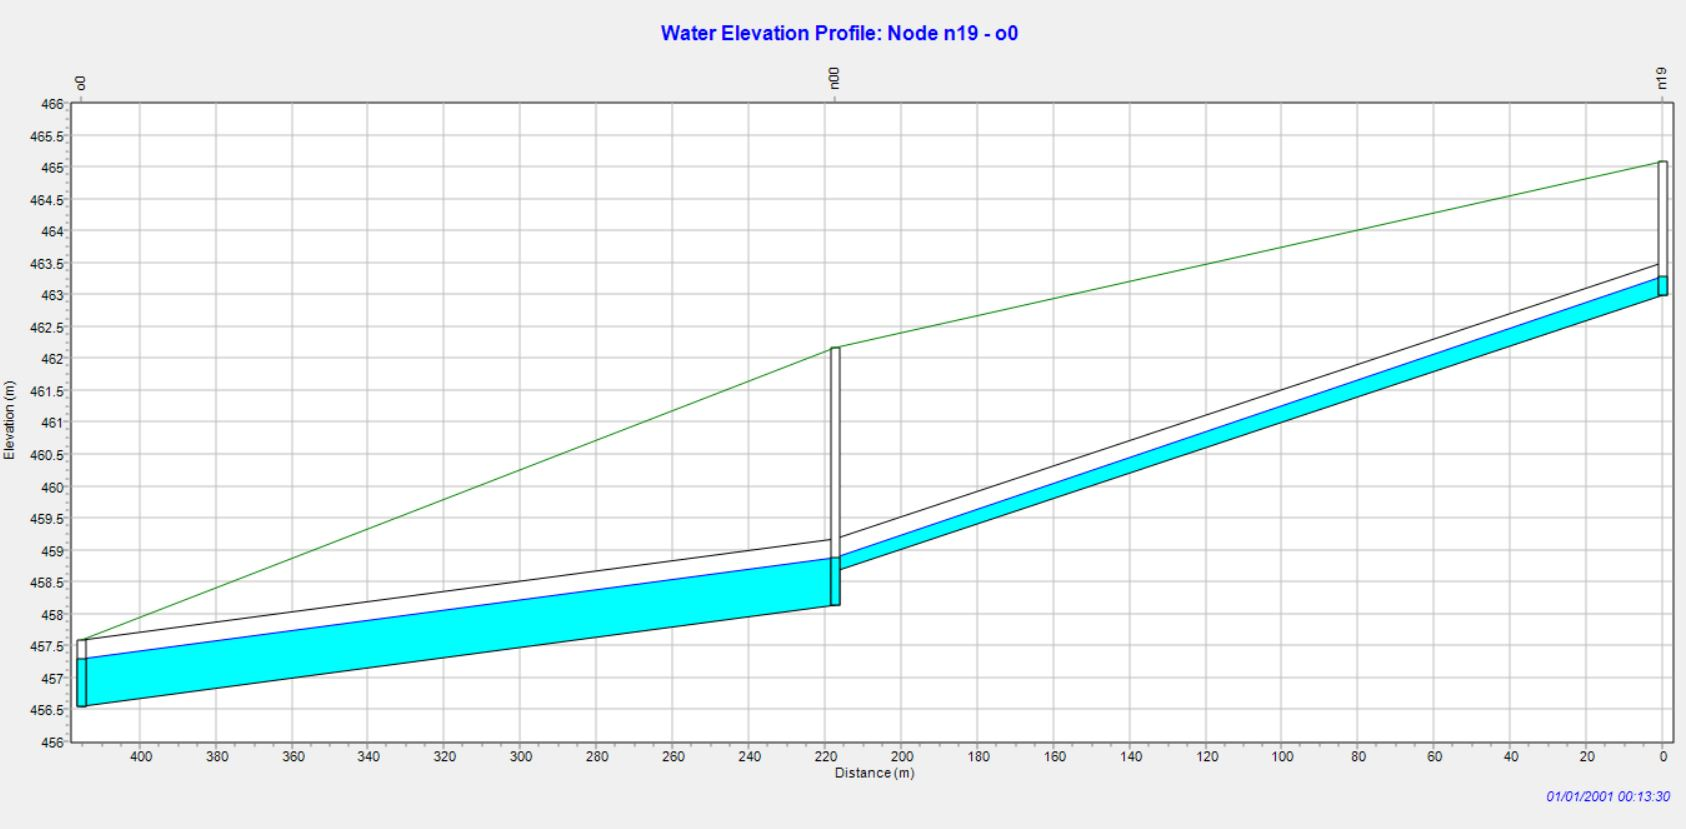
\includegraphics[width=\linewidth]{images/allineamento_cieli}
   \end{overprint}
  \end{figure}   
  \end{column}
  
  \begin{column}{.5\textwidth}
   \begin{itemize}
   \onslide<1> \item verifica del criterio di autopulizia
   \onslide<2> \item verifica della presenza di rigurgiti
   \onslide<3> \item se presenti, si procede ad allineare i cieli dei tubi
   \onslide<4> \item ricalcolo della pendenza e del diametro della condotta
   \item aggiornamento dei dati in caso di modifiche
   \end{itemize}
  \end{column}
 \end{columns}
\end{frame}

{\nologo
\begin{frame}
 \frametitle{Rete finale}
 \begin{figure}
  \centering
  \includegraphics[width=\textwidth]{images/condotte_final}
 \end{figure} 
\end{frame}
}

\section{Computo metrico estimativo}
{\nologo
\begin{frame}
 \frametitle{Schema di scavo per il calcolo delle  quote}
 \begin{figure}
  \centering
  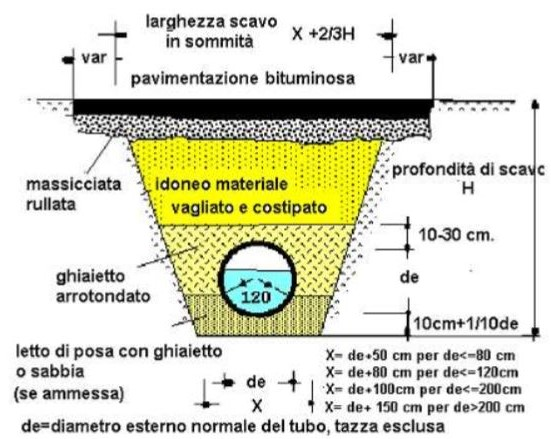
\includegraphics[height=.8\textheight]{images/scavo}
 \end{figure}
\end{frame}
}

\begin{frame}
 \frametitle{Schema pozzetto di ispezione}
 \begin{figure}
  \centering
  \includegraphics[height=.8\textheight]{images/pozzetto}
 \end{figure}
\end{frame}

{\nologo
\begin{frame}
 \frametitle{Quote finali}
 \begin{figure}
  \centering
  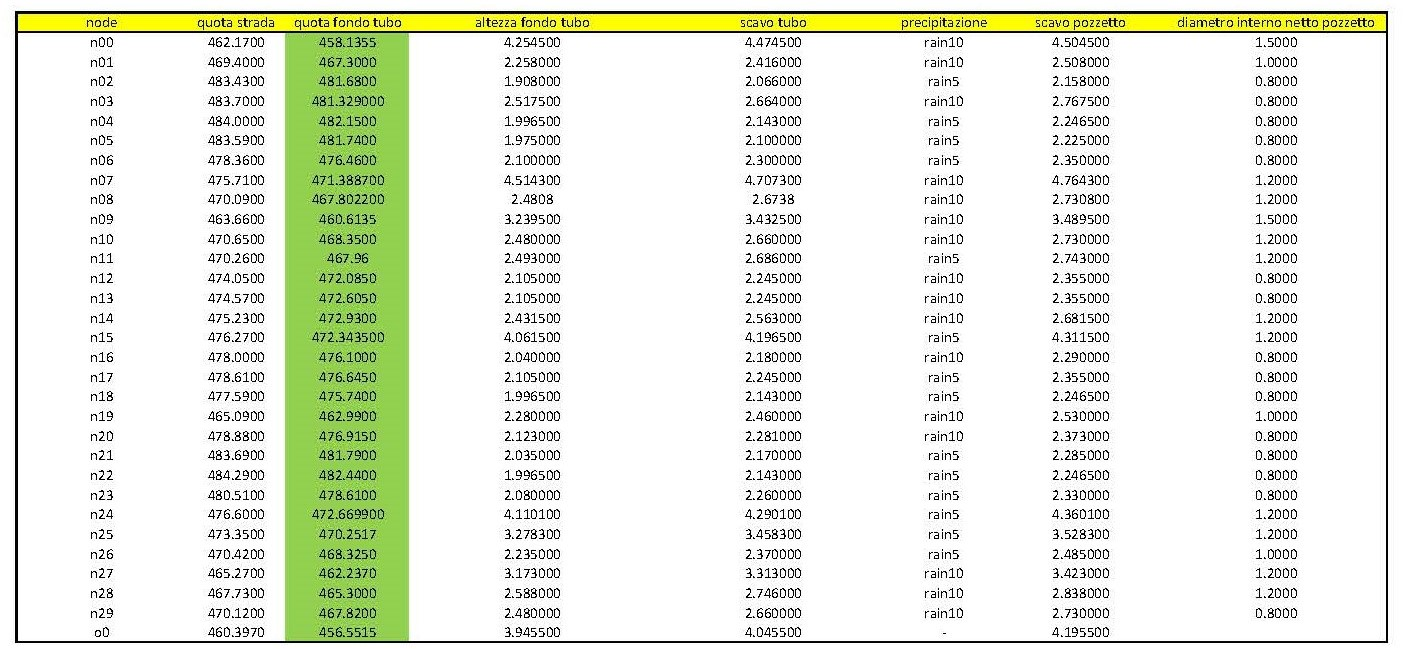
\includegraphics[width=\textwidth]{images/quote_nodi}
 \end{figure}
\end{frame}
}
{\nologo
\begin{frame}
 \frametitle{Costo dello scavo}
 \framesubtitle{Costi derivanti dall'elenco prezzi della Provincia Autonoma di Trento}
 \begin{figure}
  \centering
  \includegraphics[height=.8\textheight]{images/costo_scavo}
 \end{figure}
\end{frame}
}

\begin{frame}
 \frametitle{Costo dei pozzetti}
 \framesubtitle{Costi derivanti dall'elenco prezzi della Provincia Autonoma di Trento}
 I costi comprendono le opere di movimento terra e di posa in opera dei pozzetti, con relativo sottofondo di magrone dello spessore di $15\,cm$.
 \begin{figure}
  \centering
  \includegraphics[width=\textwidth]{images/costo_pozzetti}
 \end{figure}
\end{frame}

\begin{frame}
 \frametitle{Calcolo costi condotte}
 Poiché l'elenco prezzi provinciale contiene i prezzi di solo una parte delle condotte impiegate nel progetto della rete di fognatura pluviale, è stata fatta un'analisi dei costi interpolando i dati noti attraverso la funzione di \emph{regressione lineare}, come descritto nel relativo notebook.
 \begin{figure}
  \centering
  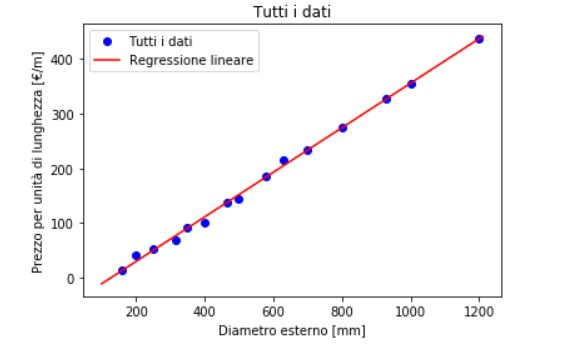
\includegraphics[height=.6\textheight]{images/interpolazione_costi_tubi.jpg}
 \end{figure}
\end{frame}


\begin{frame}
 \frametitle{Calcolo costi condotte}
 \footnotesize
 \begin{table}
  \begin{tabular}{cc}
  \toprule
  Diametro esterno [mm]& Prezzi [\euro/m] \\
  \midrule
  160                   &     $13.115787$ \\
  200                   &     $40.010000$ \\
  250                   &     $52.640000$ \\
  315                   &     $69.280000$ \\
  350                   &     $90.646501$ \\
  400                   &    $100.350000$ \\
  465                   &    $137.572985 $\\
  500                   &    $144.800000 $\\
  580                   &    $184.499470$ \\
  630                   &    $216.370000$ \\
  700                   &    $233.466237$ \\
  800                   &    $274.271876$ \\
  930                   &   $ 327.319206 $\\
  1000                  &   $ 355.883154$ \\
  1200                  &   $ 437.494431$ \\
  \bottomrule
  \end{tabular}
 \end{table}
\end{frame}

{\nologo
\begin{frame}
 \frametitle{Calcolo costi condotte}
 \begin{figure}
  \centering
  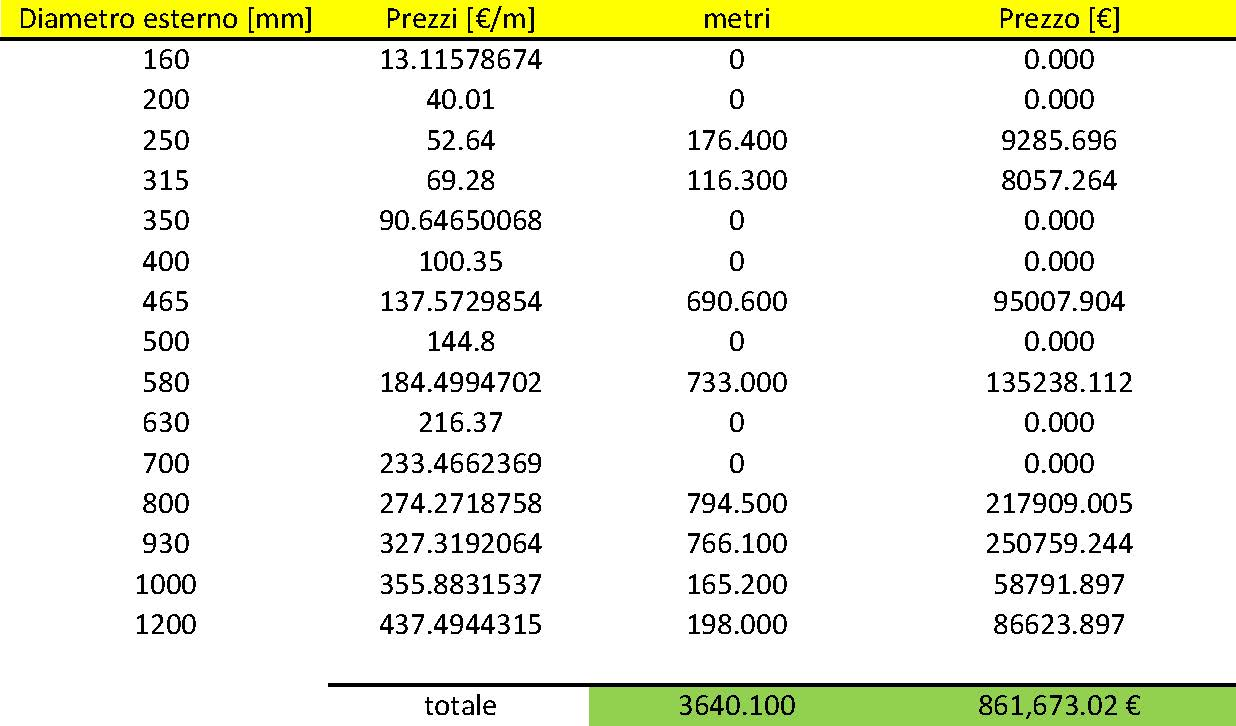
\includegraphics[width = \textwidth]{images/costo_tubi.jpg}
 \end{figure}
\end{frame}
}

\begin{frame}
 \frametitle{Costo totale dell'opera}
 Il costo totale dell'opera, tenendo conto anche di una percentuale del 5\% per gli imprevisti, risulta di
 \begin{figure}
  \centering
  \includegraphics[width=\textwidth]{images/costo_totale}
 \end{figure}
\end{frame}


\section{Fine}
{\nologo
\usebackgroundtemplate{
\tikz \node[opacity=.8] {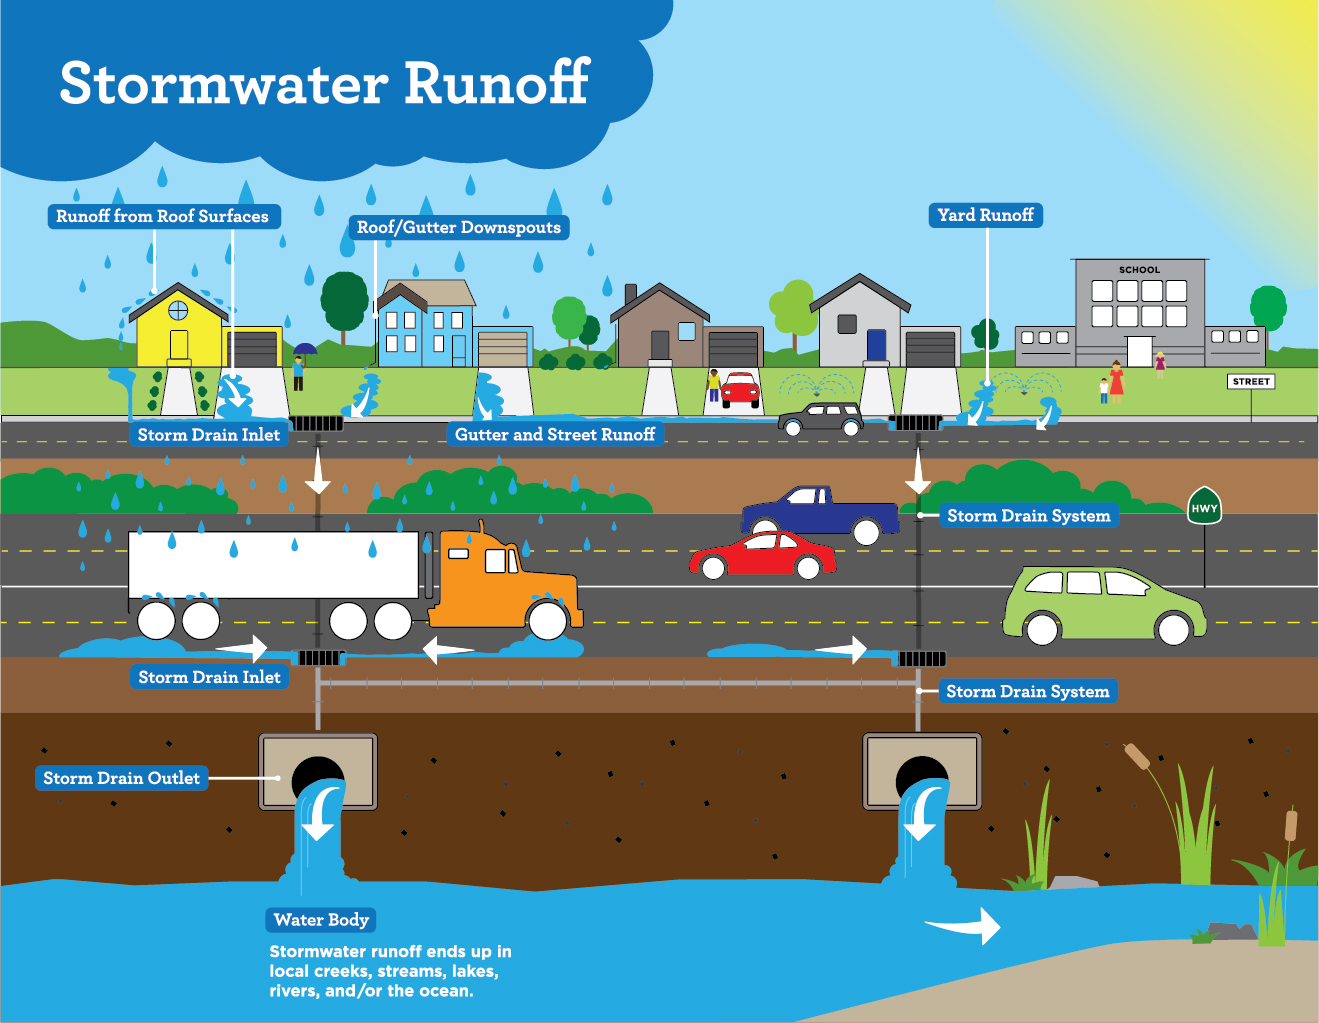
\includegraphics[width=\paperwidth]{images/titlegraphic.jpg}};}
\begin{frame}
\frametitle{Fine}
    \begin{center}
        \begin{minipage}{\textwidth}
            \begin{block}{}
                \centering\huge{Grazie per l'attenzione!}
            \end{block}
        \end{minipage}
    \end{center}

    
\end{frame}
}

\end{document}
